\documentclass[conference]{IEEEtran}
\usepackage{graphicx}


\ifCLASSINFOpdf
  % \usepackage[pdftex]{graphicx}
  % declare the path(s) where your graphic files are
  % \graphicspath{{../pdf/}{../jpeg/}}
  % and their extensions so you won't have to specify these with
  % every instance of \includegraphics
  % \DeclareGraphicsExtensions{.pdf,.jpeg,.png}
\else
  % or other class option (dvipsone, dvipdf, if not using dvips). graphicx
  % will default to the driver specified in the system graphics.cfg if no
  % driver is specified.
  % \usepackage[dvips]{graphicx}
  % declare the path(s) where your graphic files are
  % \graphicspath{{../eps/}}
  % and their extensions so you won't have to specify these with
  % every instance of \includegraphics
  % \DeclareGraphicsExtensions{.eps}
\fi
% graphicx was written by David Carlisle and Sebastian Rahtz. It is
% required if you want graphics, photos, etc. graphicx.sty is already
% installed on most LaTeX systems. The latest version and documentation
% can be obtained at: 
% http://www.ctan.org/tex-archive/macros/latex/required/graphics/
% Another good source of documentation is "Using Imported Graphics in
% LaTeX2e" by Keith Reckdahl which can be found at:
% http://www.ctan.org/tex-archive/info/epslatex/
%
% latex, and pdflatex in dvi mode, support graphics in encapsulated
% postscript (.eps) format. pdflatex in pdf mode supports graphics
% in .pdf, .jpeg, .png and .mps (metapost) formats. Users should ensure
% that all non-photo figures use a vector format (.eps, .pdf, .mps) and
% not a bitmapped formats (.jpeg, .png). IEEE frowns on bitmapped formats
% which can result in "jaggedy"/blurry rendering of lines and letters as
% well as large increases in file sizes.
%
% You can find documentation about the pdfTeX application at:
% http://www.tug.org/applications/pdftex





% *** MATH PACKAGES ***
%
%\usepackage[cmex10]{amsmath}
% A popular package from the American Mathematical Society that provides
% many useful and powerful commands for dealing with mathematics. If using
% it, be sure to load this package with the cmex10 option to ensure that
% only type 1 fonts will utilized at all point sizes. Without this option,
% it is possible that some math symbols, particularly those within
% footnotes, will be rendered in bitmap form which will result in a
% document that can not be IEEE Xplore compliant!
%
% Also, note that the amsmath package sets \interdisplaylinepenalty to 10000
% thus preventing page breaks from occurring within multiline equations. Use:
%\interdisplaylinepenalty=2500
% after loading amsmath to restore such page breaks as IEEEtran.cls normally
% does. amsmath.sty is already installed on most LaTeX systems. The latest
% version and documentation can be obtained at:
% http://www.ctan.org/tex-archive/macros/latex/required/amslatex/math/





% *** SPECIALIZED LIST PACKAGES ***
%
%\usepackage{algorithmic}
% algorithmic.sty was written by Peter Williams and Rogerio Brito.
% This package provides an algorithmic environment fo describing algorithms.
% You can use the algorithmic environment in-text or within a figure
% environment to provide for a floating algorithm. Do NOT use the algorithm
% floating environment provided by algorithm.sty (by the same authors) or
% algorithm2e.sty (by Christophe Fiorio) as IEEE does not use dedicated
% algorithm float types and packages that provide these will not provide
% correct IEEE style captions. The latest version and documentation of
% algorithmic.sty can be obtained at:
% http://www.ctan.org/tex-archive/macros/latex/contrib/algorithms/
% There is also a support site at:
% http://algorithms.berlios.de/index.html
% Also of interest may be the (relatively newer and more customizable)
% algorithmicx.sty package by Szasz Janos:
% http://www.ctan.org/tex-archive/macros/latex/contrib/algorithmicx/




% *** ALIGNMENT PACKAGES ***
%
%\usepackage{array}
% Frank Mittelbach's and David Carlisle's array.sty patches and improves
% the standard LaTeX2e array and tabular environments to provide better
% appearance and additional user controls. As the default LaTeX2e table
% generation code is lacking to the point of almost being broken with
% respect to the quality of the end results, all users are strongly
% advised to use an enhanced (at the very least that provided by array.sty)
% set of table tools. array.sty is already installed on most systems. The
% latest version and documentation can be obtained at:
% http://www.ctan.org/tex-archive/macros/latex/required/tools/


% IEEEtran contains the IEEEeqnarray family of commands that can be used to
% generate multiline equations as well as matrices, tables, etc., of high
% quality.




% *** SUBFIGURE PACKAGES ***
%\ifCLASSOPTIONcompsoc
%  \usepackage[caption=false,font=normalsize,labelfont=sf,textfont=sf]{subfig}
%\else
%  \usepackage[caption=false,font=footnotesize]{subfig}
%\fi
% subfig.sty, written by Steven Douglas Cochran, is the modern replacement
% for subfigure.sty, the latter of which is no longer maintained and is
% incompatible with some LaTeX packages including fixltx2e. However,
% subfig.sty requires and automatically loads Axel Sommerfeldt's caption.sty
% which will override IEEEtran.cls' handling of captions and this will result
% in non-IEEE style figure/table captions. To prevent this problem, be sure
% and invoke subfig.sty's "caption=false" package option (available since
% subfig.sty version 1.3, 2005/06/28) as this is will preserve IEEEtran.cls
% handling of captions.
% Note that the Computer Society format requires a larger sans serif font
% than the serif footnote size font used in traditional IEEE formatting
% and thus the need to invoke different subfig.sty package options depending
% on whether compsoc mode has been enabled.
%
% The latest version and documentation of subfig.sty can be obtained at:
% http://www.ctan.org/tex-archive/macros/latex/contrib/subfig/




% *** FLOAT PACKAGES ***
%
%\usepackage{fixltx2e}
% fixltx2e, the successor to the earlier fix2col.sty, was written by
% Frank Mittelbach and David Carlisle. This package corrects a few problems
% in the LaTeX2e kernel, the most notable of which is that in current
% LaTeX2e releases, the ordering of single and double column floats is not
% guaranteed to be preserved. Thus, an unpatched LaTeX2e can allow a
% single column figure to be placed prior to an earlier double column
% figure. The latest version and documentation can be found at:
% http://www.ctan.org/tex-archive/macros/latex/base/

\usepackage{graphicx}
%\usepackage{stfloats}
% stfloats.sty was written by Sigitas Tolusis. This package gives LaTeX2e
% the ability to do double column floats at the bottom of the page as well
% as the top. (e.g., "\begin{figure*}[!b]" is not normally possible in
% LaTeX2e). It also provides a command:
%\fnbelowfloat
% to enable the placement of footnotes below bottom floats (the standard
% LaTeX2e kernel puts them above bottom floats). This is an invasive package
% which rewrites many portions of the LaTeX2e float routines. It may not work
% with other packages that modify the LaTeX2e float routines. The latest
% version and documentation can be obtained at:
% http://www.ctan.org/tex-archive/macros/latex/contrib/sttools/
% Do not use the stfloats baselinefloat ability as IEEE does not allow
% \baselineskip to stretch. Authors submitting work to the IEEE should note
% that IEEE rarely uses double column equations and that authors should try
% to avoid such use. Do not be tempted to use the cuted.sty or midfloat.sty
% packages (also by Sigitas Tolusis) as IEEE does not format its papers in
% such ways.
% Do not attempt to use stfloats with fixltx2e as they are incompatible.
% Instead, use Morten Hogholm'a dblfloatfix which combines the features
% of both fixltx2e and stfloats:
%
% \usepackage{dblfloatfix}
% The latest version can be found at:
% http://www.ctan.org/tex-archive/macros/latex/contrib/dblfloatfix/




% *** PDF, URL AND HYPERLINK PACKAGES ***
%
%\usepackage{url}
% url.sty was written by Donald Arseneau. It provides better support for
% handling and breaking URLs. url.sty is already installed on most LaTeX
% systems. The latest version and documentation can be obtained at:
% http://www.ctan.org/tex-archive/macros/latex/contrib/url/
% Basically, \url{my_url_here}.




% *** Do not adjust lengths that control margins, column widths, etc. ***
% *** Do not use packages that alter fonts (such as pslatex).         ***
% There should be no need to do such things with IEEEtran.cls V1.6 and later.
% (Unless specifically asked to do so by the journal or conference you plan
% to submit to, of course. )


% correct bad hyphenation here
\hyphenation{op-tical net-works semi-conduc-tor}


\begin{document}
%
% paper title
\title{DSRC Challenges with Malicious Acts and its Reliability and Survivability in VANETs}


% author names and affiliations
% use a multiple column layout for up to three different
% affiliations
\author{\IEEEauthorblockN{Chihsiang Wang}
\IEEEauthorblockA{Computer Science\\
University of Idaho\\
Email: wang0162@vandals.uidaho.edu}}






% make the title area
\maketitle

% As a general rule, do not put math, special symbols or citations
% in the abstract
\begin{abstract}
Reliability and Survivability are such important for the DSRC communication, since any non-malicious or malicious acts may cause severe effects. As the DSRC applications are applying to the modern vehicles to increase the safety abilities for drivers. Every researches about to detect and correct misbehaviors are important. This paper summarized some recently researches which focus on the malicious acts especially on VANETs and its strategies to avoid or react while misbehaviors happens.

\end{abstract}

\begin{IEEEkeywords}
BSM, DSRC, VANET, Misbehaviors, System reliability and survivability.
\end{IEEEkeywords}
% no keywords




% For peer review papers, you can put extra information on the cover
% page as needed:
% \ifCLASSOPTIONpeerreview
% \begin{center} \bfseries EDICS Category: 3-BBND \end{center}
% \fi
%
% For peerreview papers, this IEEEtran command inserts a page break and
% creates the second title. It will be ignored for other modes.
\IEEEpeerreviewmaketitle



\section{Introduction}

As previous work\cite{Last-Work} has been mentioned. Vehicular Ad Hoc Networks (VANETs) are becoming more important to enhance road traffic safety. In an Ad hoc network, collection of nodes dynamically forms a network without existing infrastructures or centralized administration [1]. A VANET consists of a set of vehicles equipped with on-board units (OBUs) and a set of stationary units called road side units (RSUs), communicating each other with the ad hoc connection that are established on the fly when they are in the communication range. Providing efficient Vehicle to Vehicle (V2V) and Vehicle to Infrastructure (V2I) are the main objectives of VANETs[3]. VANET applications can be divided into two into two categories: safety applications and non-safety applications. Those applications that are critical to human life safety such as pre-crash sensing, post-crash warning, etc. are under safety application categories. Quality of Service is one of the main concerns in any type of wireless communication. In high density environment, each vehicle broadcasts message flood at a high frequency, that can easily congest the Control channel (CCH). Also, malicious acts like jamming can disable BSM works normally. Keeping CCH channel free from congestion is very important in order to ensure timely and reliable delivery of Basic Safety Messages (BSMs). The rest of this paper is organized as follows: Section 2 describes some background knowledge such as Waht Basic Safety Messages and DSRC is and what are the challenges associated with this technology. Section 3 presents types of malicious acts to DSRC system and its strategies. Section 4 concludes this paper.


\section{Background}
\subsection{Vehicular Ad-hoc Network}
In VANET (Vehicular Ad-hoc Network), vehicles equipped with short range radios communicate with each other (Vehicle-to-Vehicle - V2V) and with the road side infrastructure (Vehicle-to-Infrastructure - V2I) to enable range of applications from Internet access and driver assistance to transportation safety and emergency response. Network topology in VANET changes frequently due to high node mobility. V2V and V2I operates in the 75 MHz Dedicated Short Range Communication (DSRC) spectrum. The spectrum is allocated within 5.85 - 5.925 GHz band which is divided into one control channel and six service channels. All vehicles will broadcast their state information such as location, speed, vehicle size, etc., frequently in Basic Safety Message (BSMs). According to the standards, each vehicle should transmit one BSM every 100 milliseconds in DSRC.

\begin{figure}[h]
  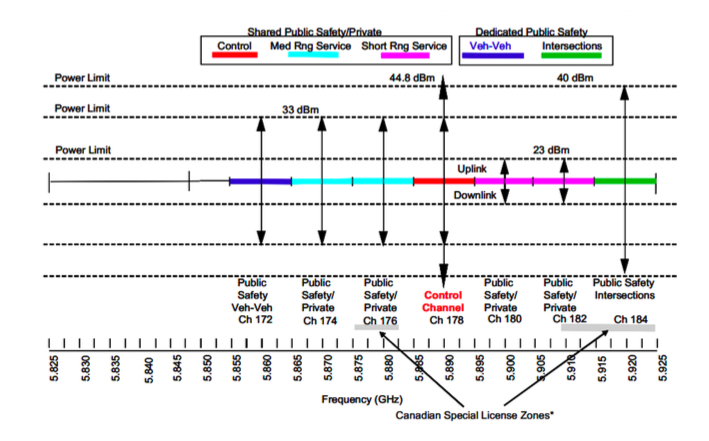
\includegraphics[width=\linewidth]{Fig-Channel-power.png}
  \caption{DSRC channels and Power Limit[3]}
  \label{fig:channel}
\end{figure}

\subsection{Dedicated Short Range Communication}
DSRC uses IEEE 802.11p as its PHY and MAC layer, which is, a modified standard of the IEEE 802.11e with QoS (Quality of Service) at the MAC layer and basically same PHY layer defend for 802.11a but with halved transmission rate . Yet the communication speed and the range are improved. According to \cite{W2010}, 802.11p provides longer duration and faster communication speed between units. Besides, the loss of packet is just half compared with 802.11a. But the performance, efficiency and reliability are still limited in the real life, since there are several challenges can effect DSRC safety. That is, high speed mobile, busy traffics between buildings or intersections, malicious attacks and more. DSRC systems are based on the orthogonal frequency division multiplexing (OFDM) systems. OFDM systems are well known for their abilities to combat inter symbol interference (ISI) in time-invariant, frequency- selective channels[8]. In this paper we are going to note some malicious acts which may affect DSRC safety.
In U.S. Federal Communications Commission (FCC) has allocated 75 MHz DSRC spectrum in the 5.9 GHz band. The spectrum consists of one control channel (CCH) and six service channels (SCHs) to be used by Intelligent Transportation Systems (ITS) as shown in Figure 1.

\begin{figure}[h]
  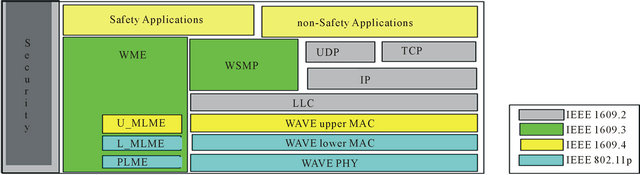
\includegraphics[width=\linewidth]{DSRC_Standard.jpg}
  \caption{Physical IP Users}
  \label{fig:User}
\end{figure}

\subsection{Basic Safety Message}
The Basic Safety Message (BSM) is used in multiple safety applications in each vehicle. These applications are largely independent of each other, but all make use of the incoming stream of BSMs from surrounding (nearby) vehicles to detect potential events and dangers\cite{BSM}. BSM is defined by the standard ASE J2735, every mobile keep updating and sending this message every 100 micro seconds over the WSM channel. Nearby OBUs and RSUs can detect the broadcast message and process it if the format is fit its safety applications. A temporary value in the message body allows correlating BSMs to a specific vehicle for short periods of time. The rationale of the BSM is for create a most statistically frequent message seen over the airwaves.
\begin{figure}[h]
  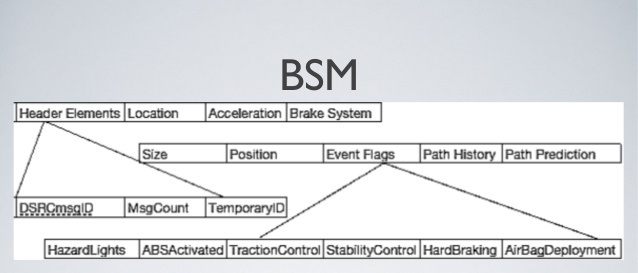
\includegraphics[width=\linewidth]{BSM.jpg}
  \caption{BSM}
  \label{fig:BSM}
\end{figure}

There are two sections consisted in the BSM. Part 1 is always necessary to be sent during the broadcast, which combined DER encoding and some BLOB encoding, also it contains node's position, motion, time and basic status. Part 2 contains vary optional data within, safety applications may add on the extra data with it if that is useful for the processing.\cite{BSM}

\section{Misbehaviors}
In order to meet performance goals, it is widely agreed that VANETs rely on heavily node to node communication. Since the system concern the speed of quick data transmission, it is also bring the issue that an easy access system may have more difficult security goal of data validation. \cite{NICE}
\subsection{Misbehaving Nodes}
A bad or malicious data node(vehicle) in VANETs may try to send fake message such include wrong event reports, such as non-exist traffic jam, car accident and any of information content in the Basic Safety Messages like speed, location, status and many others. Wrong messages via malicious nodes can cause severe damaging if there is no strategies to detect and correct the nodes. In the VANETs, these mistakes are called misbehaviors no matter it's rational or malicious. Here we are classify the misbehaving nodes by it abilities before we get into the rationale of misbehavior nodes.
\subsubsection{Rational and Malicious}
Usually attackers can be divide into two groups by their objectives. Malicious attackers are purely enjoy to see the damaging of the system, rather than rational attackers, they don't consider benefit, cost or consequences. In some situations malicious attackers are more dangerous  because we can't predict their intentions. \cite{40}
\subsubsection{Outsider and Insider}
Outsider means those node out of the network, which has no legitimate access to the system network. In opposite the insider is the node which accepted by the system network. Usually outsiders are harder to effect the network rather than insider which may have certain control of cryptographic materials.\cite{32} 
\subsubsection{Single and Multiple}
The adversarial nodes can be work as single or multiple in the network. For multiple adversaries every nodes can work independently or together. If the group of adversaries are fixed during the attack, then they can be viewed as non-adaptive adversary\cite{NICE}. It is also possible that the members in the adversary group change over time. The main adversary in the group can choose which node to compromise. It makes the adversary group an adaptive adversary group \cite{Sta}. Although the type of collective adaptive adversary exists in theory, it is difficult to become real threat in VANETs. Because in the VANETs, the topology of nodes changes rapidly.


\subsection{Type of Attacks}
As VANETs is part of network system, it also face some similar security attacks. In this section we classify the attack types into three groups by their target. 
\subsubsection{Attacks target Messages in VANETs}
In VANETs, there is a special type of message tempering called message suppression attack\cite{35}. This attack is done by delay the broadcasting of some messages so that the attacker
can get benefit from it. Network accidental failures are not avoidable, such like omission failure, commission failure and timing failure. With exceeded fault tolerance amount nodes, it can lead to difficult of avoid the Byzantine failure. With these malicious nodes and the failure of node communication protocol, malicious acts may modify, delete the safety messages for reliable nodes. However, Byzantine fault tolerance problem is hard to deal with in VANETs due to its highly dynamic network.
\begin{figure}[h]
  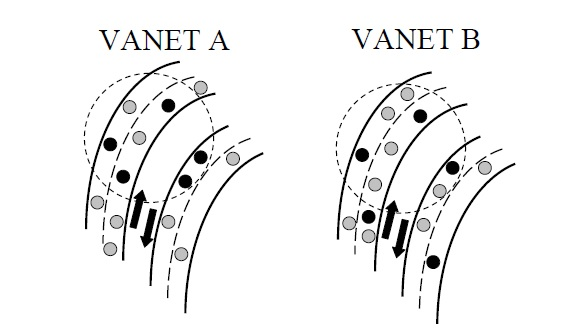
\includegraphics[width=\linewidth]{Control.jpg}
  \caption{Black nodes represent as malicious nodes. Gray circles represent reliable nodes. Dash line circle represent the communication range}
  \label{fig:Attack2}
\end{figure}
As figure 4, VANETs A shows the example that the colluding adversaries (indicated by the black circles) are successful in convincing the honest node (shown in gray at the center of the circle) of false data, but in a VANET it is difficult to maintain such a configuration for any significant duration\cite{Way}.


\subsubsection{Attacks target Users in VANETs}
In the VANETs, every node content with personal privacy, the malicious attacker may catch the information from every node in the network. Usually there are many kinds of privacy information may directly effect the network security. One of the most important information is the node's ID. ID disclosure is dangerous if the attacker catch the safety node access of the network, it will turns to unreliable node and may do modification and overwhelm the original resource. The node ID is always related to the public key correlation, so one of the attack type is that the attacker set up two receivers on a predictable pathway, then they can analyze and steal the public key for the network access in the node has not change the key in this interval. Anonymous changeable keys may help to fix this issue, however, it will bring another difficult that every time when the key changed, the certification will need to be  recheck again. So the revocation of keys and certificates is difficult issue in VANETs. Also, there are many other valuable information from the target users like location tracking, and all of these information should be well protect in case of malicious usages. 
\begin{figure}[h]
  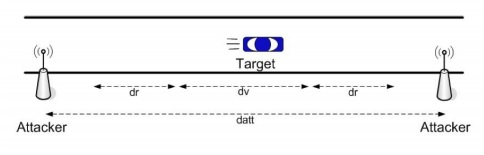
\includegraphics[width=\linewidth]{Attack2.jpg}
  \caption{Sample of attacks}
  \label{fig:Attack2}
\end{figure}


\subsubsection{Attacks target Network in VANETs}
Denial of Service (DoS) is one of the most common way to disable a system by sending bunch of flood requests. In VENETs it can target a single node or focus on part of network, Dos can be done by cover a particular node(vehicle) resource or Jamming the channel and cause the malicious CCH(Congestion Control Channel). As a reliability concern for the network communication, jamming need to be considered with Constant Jamming and Random Jamming. Attackers may also choose to target routing protocol applied in the network [10]. \cite{Sta} mentioned that there are still no widely agreed which type of routing protocol should be used in VANETs. It may be harder for attack to conduct wormhole attack than in other network system since VANETs is highly dynamic. In the research \cite{Way}, they design a method to detecting and correcting errors that have been maliciously introduced into data in a VANET. ``The approach relies on using sensor data, collected by nodes in the VANET, shared with immediate neighbors, and propagated to a neighboring region''\cite{Way}.

And there are many other network attacks which also can be effect in the VANETs like Sybil attack, Bogus message attack, Eaves Dropping, Masquerading, Worm Hole, Message Suppression attack.\cite{S-9}

\section{Conclusion}
In this paper we summarized and classify the malicious acts for the VANETs. As most of researches mentioned, while nodes in the VANETs are highly dynamic and hard to apply on formal data communication security technique, so the Byzantine failures problem may be a highly concern question. As the \cite{Sta} shows, some recent DSRC researches are looking for the strategies to increase Reliability and Survivability for DSRC communication.  However, still there exists many challenges related brute force malicious acts. Reliability of the DSRC safety application is the major thing that should never be compromised since it related to the safety of life. But if it is almost impossible to avoid mistakes happened, the system should consider what to react rather than how to avoid, that is, survivability.  
\begin{thebibliography}{1}

	\bibitem{VeMAC}
	H. Omar , W. Zhuang and L. Li {\em VeMAC: A TDMA-based MAC protocol for reliable broadcast in VANETs}, IEEE Trans. Mobile Comput.,  vol. 12,  no. 9,  pp.1724 -1736 2013.	
	
	\bibitem{FINA2014}
	A. Serageldin, and A. Krings, {\em The Impact of Dissimilarity and Redundancy on the Reliability of DSRC Safety Applications}, Proc. Tenth International Symposium on Frontiers of Information Systems and Network Applications, (FINA 2014), Victoria, Canada, May 13-16, 2014.
	
	\bibitem{NIMS2014}
	A. Serageldin, and A. Krings, {\em The Impact of Redundancy on DSRC Safety Application Reliability under Different Data Rates}, Proc. 6th International Conference on New Technologies, Mobility and Security, (NTMS 2014), Dubai, March 30 - April 2, 2014.
	
	
\bibitem{Sta}
Philippe G.; Dan G.; Jessica S. {\em Detecting and Correcting Malicious Data in VANETs} in Palo Alto Research Center, 2014
	
	\bibitem{W2010}
	W. Lin, et. al., A comparison of 802.11a and 802.11p for V-to-I
communication: a measurement study, ICST QShine, 2010.
	

	\bibitem{40}
	Maxim Raya and Jean-Pierre Hubaux. {\em Securing vehicular ad hoc networks}.
Journal of Computer Security, 15(1):39–68, 2007
	
	\bibitem{32}
	P. Papadimitratos, V. Gligor, and J-P. Hubaux. {\em Securing vehicular
communications-assumptions, requirements, and principles}. In Workshop on
Embedded Security in Cars (ESCAR), volume 2006, 2006.



	\bibitem{S-2}
	A. Serageldin, and A. Krings, {\em The Impact of Redundancy on DSRC Safety Application Reliability under Different Data Rates}, Proc. 6th International Conference on New Technologies, Mobility and Security, (NTMS 2014), Dubai, March 30 - April 2, 2014.
	
	\bibitem{S-3}
	Jianhua He, et. al. {\em Adaptive Congestion Control for DSRC Vehicle Networks}, IEEE COMMUNICATIONS LETTERS, VOL. 14, NO. 2, FEBRUARY 2010
	
	\bibitem{S-6}
	Xiaomin Ma, et. al. {\em Performance and Reliability of DSRC Vehicular Safety Communication: A Formal Analysis}, IEEE Commun. Mag., 2009.
	
	\bibitem{S-7}
	Nabih Jaber. {\em Performance Enhancement of the OFDM-Based DSRC System Using Frequency-Domain MAP Equalization and Soft-Output Demappers}, University of Windsor, 2009.
	\bibitem{S-8}
	Pelechrinis, K.; Iliofotou, M.; Krishnamurthy, S.V., "Denial of Service Attacks in Wireless Networks: The Case of Jammers," in Communications Surveys \& Tutorials, IEEE , vol.13, no.2, pp.245-257, Second Quarter.

	\bibitem{S-9}
Praba, V.L.; Ranichitra, A., "Isolating malicious vehicles and avoiding collision between vehicles in VANET," in Communications and Signal Processing (ICCSP), 2013 International Conference on , vol., no., pp.811-815, 3-5 April 2013
doi: 10.1109/iccsp.2013.6577169

	\bibitem{Last-Work}
	Anup, C.; Chihsiang W., \''DSRC Challenges and its Reliability during Congestion in Intelligent Transportation System\'', in CS520 Semester Project, 2015 Computer Science University of Idaho

\bibitem{BSM}
	SAE International {\em DSRC Implementation Guide A guide to users of SAE J2735 message sets over DSRC}, 2014.

\bibitem{NICE}
	Shuxian L., {\em Analysis and detecting of misbehaviours in VANETs}, 2014.

\bibitem{35}
B. Parno and A. Perrig. {\em Challenges in securing vehicular networks}. In Workshop
on hot topics in networks (HotNets-IV), pages 1–6, 2005.

\bibitem{Way}
Philippe Golle, Dan Greene, and Jessica Staddon. 2004. {\em Detecting and correcting malicious data in VANETs.} In Proceedings of the 1st ACM international workshop on Vehicular ad hoc networks (VANET '04).
\end{thebibliography}




% that's all folks
\end{document}


